\documentclass[11pt,a4paper,twoside,french,svgnames]{report}
\usepackage[utf8]{inputenc} % force the use of utf8
\usepackage[T1]{fontenc} % font encoding, allows accents (T1 font encoding is an 8-bit encoding)
\usepackage[top=2.5cm,bottom=2.5cm,outer=2.5cm,inner=2.5cm]{geometry} % http://tex.stackexchange.com/questions/62311/a4paper-where-should-i-declare-it-in-document-class-or-geometry // another option: papersize={21cm,29.7cm}
\usepackage[french]{babel} % translate everything in the desired language: table of contents, etc. 'english' can be replaced with 'francais'
\usepackage{graphicx} % images management
\usepackage{wrapfig} % floating images
\usepackage[format=plain,labelfont=bf,font=small,justification=centering,margin=10pt]{caption} % allow multiline captions in figures,
\usepackage{float} % allow \begin{figure}[H] and \begin{table}[H] (to really force positionning, unlike h!)
\usepackage{array} % allow arrays
\usepackage[super]{nth} % allow to write \nth(1) to write 1st, etc
\usepackage{fancyhdr} % headers/footers management (overrides empty, plain and headings)
\usepackage{upquote} % without this, lslisting replace vertical singles quotes with curved ones
\usepackage{listings} % code insertion (MUST BE WRITTEN AFTER BABEL)
\usepackage[
            backend=biber,
            style=numeric,
            sorting=none, % nty = name title year
            url=true, % always show url when provided
            ]{biblatex}
%\usepackage{pdfpages} % include PDF documents
\usepackage{enumitem} % for /setlist
\usepackage{color,soul} % add some colors and hightlight
\usepackage{xcolor} % more colors
\usepackage{afterpage} % allow to execute command after the current page ends
\usepackage[hidelinks,
            colorlinks  = false, % no borders, colors enabled
            anchorcolor = blue,
            linkcolor   = black, % links in table of contents
            urlcolor    = blue,
            citecolor   = blue,
            breaklinks  = true]{hyperref}
\newcommand{\MYhref}[3][blue]{\href{#2}{\color{#1}{#3}}}%

% List settings
\setlist{itemsep=.5em}
\setlist[itemize,2]{label={$\bullet$}} % use bullets for nested itemize in level 2

% REQUIRE
% \usepackage{color}
% \usepackage{listings} % (MUST BE WRITTEN AFTER BABEL)

% General colors
\definecolor{comment}{rgb}{0.12, 0.38, 0.18 } % adjusted, in Eclipse: {0.25, 0.42, 0.30 } = #3F6A4D
\definecolor{keyword}{rgb}{0.2, 0.2, 0.8}
\definecolor{string}{rgb}{0.06, 0.10, 0.98} % #101AF9

% Language-specific colors
% JavaScript
\definecolor{darkgray}{rgb}{.4,.4,.4}
%\definecolor{purple}{rgb}{0.65, 0.12, 0.82}

% hack to force UTF-8 compatibility (for french only)
\lstset{
       extendedchars=true,
       literate={à}{{\`a}}1 {â}{{\^a}}1 %                         lettre a
                {À}{{\`A}}1 {Â}{{\^A}}1 %                         lettre A
                {ç}{{\c{c}}}1 %                                   lettre c
                {Ç}{{\c{C}}}1 %                                   lettre C
                {é}{{\'e}}1 {è}{{\`e}}1 {ê}{{\^e}}1 {ë}{{\"e}}1 % lettre e
                {É}{{\'E}}1 {È}{{\`E}}1 {Ê}{{\^E}}1 {Ë}{{\"E}}1 % lettre E
                {î}{{\^i}}1 {ï}{{\"i}}1 %                         lettre i
                {Î}{{\^I}}1 {Ï}{{\"I}}1 %                         lettre I
                {ô}{{\^o}}1 %                                     lettre o
                {Ô}{{\^O}}1 %                                     lettre O
                {œ}{{\oe}}1 %                                     lettre oe
                {Œ}{{\OE}}1 %                                     lettre OE
                {ù}{{\`u}}1 {û}{{\^u}}1 {ü}{{\"u}}1 %             lettre u
                {Ù}{{\`U}}1 {Û}{{\^U}}1 {Ü}{{\"U}}1 %             lettre U
}

% General rules
\lstset{
  rulecolor=\color{black!50},
  backgroundcolor = \color{blue!10},
  numbers=none, %left % display line numbers
  showspaces=false,
  showtabs=false,
  breaklines=true,
  showstringspaces=false,
  breakatwhitespace=false,
  commentstyle=\color{comment},
  keywordstyle=\color{keyword},
  stringstyle=\color{string},
  basicstyle=\ttfamily,
  extendedchars=true,
  emph=[2]{In},
  emphstyle=[2]\color{black!70},
  morecomment=[l][\color{blue}]{Out},
  frame=single,
  frameround=tttt,
  framerule=0.3pt,
  framesep=4pt,
  belowcaptionskip=2.1pt
}

% % Define "Javascript" because lstlistings doesn't know it
% Taken from https://gist.github.com/Geruhn/3d21f60a869457373d84
\lstdefinelanguage{javascript}{
  keywords={break, case, catch, continue, debugger, default, delete, do, else, false, finally, for, function, if, in, instanceof, new, null, return, switch, this, throw, true, try, typeof, var, void, while, with},
  morecomment=[l]{//},
  morecomment=[s]{/*}{*/},
  morestring=[b]',
  morestring=[b]",
  ndkeywords={class, export, boolean, throw, implements, import, this},
  %keywordstyle=\color{blue}\bfseries,
  ndkeywordstyle=\color{darkgray}\bfseries,
  identifierstyle=\color{black},
  %commentstyle=\color{purple}\ttfamily,
  %stringstyle=\color{red}\ttfamily,
  sensitive=true
}

% Usage: \javascript
\newcommand{\javascript}{\lstset{
  language=javascript,
  title={{\setlength{\fboxsep}{1pt}\fcolorbox{orange}{yellow!20}{\sffamily\scriptsize
              \textcolor{gray!10}{\_}JavaScript\textcolor{gray!10}{\_}}}}
  }
}

% Usage: \code{My title}
\newcommand{\code}[1]{\lstset{
  language=,
  title={{\setlength{\fboxsep}{1pt}\fcolorbox{orange}{yellow!20}{\sffamily\scriptsize
              \textcolor{gray!10}{\_}{#1}\textcolor{gray!10}{\_}}}}
  }
}

% Usage: \sql
\newcommand{\sql}{\lstset{
  language=SQL,
  title={{\setlength{\fboxsep}{1pt}\fcolorbox{orange}{yellow!20}{\sffamily\scriptsize
              \textcolor{gray!10}{\_}SQL\textcolor{gray!10}{\_}}}}
  }
}

% Usage: \fakeshell
\newcommand{\fakeshell}{\lstset{
  language=bash
  }
}

\newcommand{\perl}{\lstset{
  language=perl
  }
}

\newcommand{\xml}{\lstset{
  language=xml
  }
}

% REQUIRES
% Nothing

% Redefine chapter titles: only display the title and remove useless blank space
% Original "/usr/share/texlive/texmf-dist/tex/latex/base/report.cls" edited
\makeatletter
  \def\@makechapterhead#1{% chapter{}
  \vspace*{0\p@}% 50 before
  {\parindent \z@ \raggedright \normalfont
    %\ifnum \c@secnumdepth >\m@ne
    %    \huge\bfseries \@chapapp\space \thechapter
    %    \par\nobreak
    %    \vskip 20\p@
    %\fi
    \interlinepenalty\@M
    \Huge \bfseries \thechapter\quad #1   
    \vskip 40\p@
  }}
  \def\@makeschapterhead#1{% chapter*{}
  \vspace*{0\p@}% 50 before
  {\parindent \z@ \raggedright
    \normalfont
    \interlinepenalty\@M
    \Huge \bfseries  #1\par\nobreak
    \vskip 40\p@
  }}
\makeatother
% REQUIRES
% \usepackage{fancyhdr} % headers/footers management (overrides empty, plain and headings)

% THE ORDER IS REALLY IMPORTANT, OTHERWISE IT WILL BREAK THINGS

% 1.
% Redefines the existing 'plain' style, (because 'chapter' and \tableofcontents ignores the page style currently in effect for their first page)
\fancypagestyle{plain}{
    % Took from: http://anorien.csc.warwick.ac.uk/mirrors/CTAN/macros/latex/contrib/fancyhdr/fancyhdr.pdf
    \fancyhead[LO,RE]{\slshape \leftmark}
    \fancyhead[LE,RO]{\slshape \rightmark}

    % Footers
    \renewcommand{\footrulewidth}{0.4pt}
    \fancyfoot[C]{Rapport de TD -- Steve \textsc{Lagache} \& Romain \textsc{Pellerin}}
    \fancyfoot[LE,RO]{\ifdefined\thepage \thepage \fi} % to be used with \pagenumbering{gobble} % no numerotation
    % \fancyfoot[LE,RO]{\ifnum\thepage>0 \thepage \fi} % to be used with %\addtocounter{page}{-4} % numerotation begins at 1 + (-4)
}

% 2.
\pagestyle{plain}

% 3.
% http://tex.stackexchange.com/questions/111223/markboth-is-not-working-when-using-chapter-and-section
% Took from : http://ftp.snt.utwente.nl/pub/software/tex/macros/latex/contrib/fancyhdr/fancyhdr.pdf
\renewcommand{\chaptermark}[1]{\markboth{}{\MakeUppercase{\thechapter.\ #1}}}
\renewcommand{\sectionmark}[1]{}

% NORMALLY
% \renewcommand{\chaptermark}[1]{\markboth{\MakeUppercase{\thechapter.\ #1}}{}}
% \renewcommand{\sectionmark}[1]{\markright{\thesection.\ #1}}
 % To be edited to change the header and footer

\title{Rapport de TD}
\author{Steve LAGACHE et Romain PELLERIN}
\date\today
\setcounter{tocdepth}{2} % ToC depth

\pagenumbering{arabic} % re-enable numering

\begin{document}
\thispagestyle{empty} % only applies to this page
\begin{center}

\includegraphics[height=3cm]{images/logo-utc.png}

\vspace{4cm}

\noindent{\LARGE\MYhref[black]{http://www.utc.fr/}{Université de Technologie de Compiègne}}

\vspace{1cm}

{\large Génie Informatique}

\vspace{3cm}
\noindent\fbox{
\begin{minipage}{.9\textwidth}
\begin{center}
    \vspace{0.3cm}\Large{Rapport de TD}\\
    \vspace{0.3cm}\LARGE{\textbf{LO17}}\vspace{0.3cm}\\
\end{center}
\end{minipage}}

\vspace{3cm}

\begin{tabular}{>{\hfill\arraybackslash}p{5cm}p{5cm}}
%\hline
    \multicolumn{2}{c}{\textbf{Steve \textsc{LAGACHE} \& Romain \textsc{PELLERIN}}}\\\\
%\hline
    \multicolumn{2}{c}{Chargé de TD : Pierre \textsc{Morizet-Mahoudeaux}}\\\\
%\hline
    \multicolumn{2}{c}{Printemps 2016 (P16)}\\
%\hline

\end{tabular}
\vfill

{\footnotesize Dernière mise à jour: \today}
\end{center}


\tableofcontents

\chapter{TD1: Structuration}

L'objectif de ce TD était de s'initier au ``\textit{parsing}'' en Perl. Nous avions un peu plus de 300 pages HTML contenant toute un article issu d'un même site scientifique. Il nous fallait extraire des données ``uniques'' comme le numéro de l'article ou sa rubrique, et des données présentes une (parfois zéro) ou plusieurs fois, comme les paragraphes du texte principal ou les images présentes.

\section{Méthodologie employée}

Pour la totalité des éléments à récupérer, nous avons utilisé des \textit{regex} (sauf pour le nom du fichier que nous récupérerions dans \lstinline{$ARGV}).

Pour produire notre XML, nous avons décidé de tout afficher sur la sortie standard. Il s'agira ensuite de rédiriger cette sortie standard dans un fichier grâce à l'opérateur \lstinline{>} d'Unix.

\subsection{Repérer un élémént d'intérêt}

Pour chaque élément unique qu'il nous fallait récupérer, nous avons essayer de trouver la structure de balises HTML voisinante la plus proche possible qui soit unique. Pour cela, nous avons beaucoup fait appel à la structure \lstinline{.*?} (n'importe quel caractère zéro, une ou plusieurs fois) dans son mode \textit{lazy}. Par exemple, pour le numéro, la structure HTML autour était suffisant simple pour ne pas utiliser ``n'importe quel caractère'' :

\perl
\begin{lstlisting}
$body=~/<span class="style95" style="color:inherit">(\d+)<\/span><\/a>/;
\end{lstlisting}

Tandis que nous en avons eu besoin pour la partie contact :

\begin{lstlisting}
$body =~ /Pour en savoir plus, contacts :.*?<p class="style44"><span class="style85">(.*?)<\/span>/s;
\end{lstlisting}

\subsection{Lecture du contenu d'un fichier}

Nous avons été capables de récuperer le contenu d'un fichier passé en argument grâce à une boucle sur l'opérateur ``diamant''. Fondalement, cet opérateur permet de boucler sur chaque ligne de ``l'\textit{input}''. Nous avons donc simplement récupéré chaque ligne du fichier et avons concaténé ces lignes à une variable \lstinline{$body} initialisée à une chaîne de caractères vide.

\subsection{Lecture du contenu de plusieurs fichiers}

Pour pouvoir récupérer toutes les lignes de chaque fichier tout en dissociant les fichiers, nous avons du opter pour une technique légèrement différente.

\begin{enumerate}
  \item Nous créons une tableau.
  \item Chaque ``case'' du tableau sera une variable similaire à \lstinline{$body} dont nous avons parlé au-dessus: elle contiendra toutes les lignes \textbf{d'un seul fichier}.
  \item Grâce à l'opérateur diamant, nous bouclons sur toutes les lignes de l'\textit{input}.
  \item Nous sommes capable de savoir à tout instant quel fichier nous sommes en train de lire grâce à la variable \lstinline{$ARGV}.
  \item Une fois que nous avons récupéré tous les différents documents dans chaque case du tableau, nous commençons à boucler sur ce tableau de la même manière que nous le faisions pour un seul fichier.
\end{enumerate}

\perl
\begin{lstlisting}
@htmls;
while (<>) {
  $fichier = $ARGV;
  $fichier=~s/.*\///g;
  if (!defined(@htmls{$fichier})) {
    $htmls{$fichier} = $_;
  }
  else {
    $htmls{$fichier} .= $_;
  }
}

print "<corpus>\n";
while (($fichier,$html) = each(%htmls)) {
  print "<bulletin>\n";
  ...
  print "</bulletin>\n";
  }
print "</corpus>\n";
\end{lstlisting}

\section{Commandes Unix}

\subsection{Génération du XML}

Voici la commande Unix utilisée pour récupérer la sortie standard de notre programme et la rediriger dans un fichier XML. Il faut également préciser que nous avons rendu notre programme exécutable grâce à \lstinline{chmod}. De plus, nous utilisons le script \lstinline{convert.pl} pour convertir les entités HTML en caractère Unicode.

\fakeshell
\begin{lstlisting}
./td1.pl BULLETINS/*.htm | perl convert.pl > output.xml
\end{lstlisting}

\subsection{Vérification du nombre d'images}

Nous avons également utilisé quelques commandes Unix supplémentaires dans le but de vérifier que nous récupérerions bien le nombre exactes d'images présentes dans les articles. Par exemple, nous avons utilisé \lstinline{grep} dans son mode \textit{regex}.

\begin{lstlisting}
./td1.pl BULLETINS/*.htm | perl convert.pl > output.xml && { grep "<image>" output.xml } | wc -l && echo "Images parsées en Perl" && { grep -aoE "streaming.+?\.jpg" BULLETINS/*.htm && grep -aoE "<img.*?www\.bulletins-electroniques\.com\/Resources_fm\/actualites.*?\.jpg" BULLETINS/*.htm } | wc -l && echo "Images dans les fichiers d'origine";
\end{lstlisting}

\begin{figure}[H]
  \centering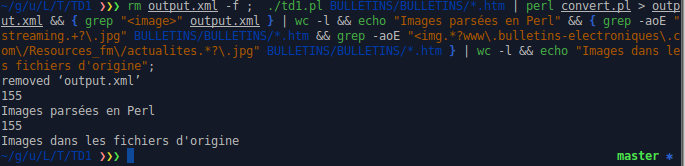
\includegraphics[width=1.00\textwidth]{images/output_td1.png}
  \caption{Résultat de la commande}
\end{figure}


%\chapter{Conclusion générale}

\section{OpenGL ou Unity}

La plus grosse problématique du projet aura été le choix entre Unity et OpenGL. Nous étions initalement partis sur du développement en OpenGL mais heureusement, en début d'année 2015, Unity a rendu son moteur totalement gratuit, nous permettant ainsi de pouvoir l'utiliser. Nous nous en sommes rendus compte peu de temps après le début du projet et avons ainsi changé de technologie. Nous avons tout de même eu le temps d'essayer OpenGL et il s'était avéré que le développement aurait été bien trop dur et presque impossible. Effectivement, nous ne connaissions pas cette technologie et la contrainte de temps (un semestre) ne nous aurait pas permis de l'appréhender.

\section{Problèmes}

Un autre problème aura été l'utilisation du SDK de Google. Au départ nous ne savions pas comment faire déplacer le joueur, nous étions donc partis sur l'utilisation d'une \textit{library} tierce, Dive. Or il s'est avéré que cette \textit{library} souffrait d'un bug au niveau du gyroscope. Nous avons finalalement réussi à utiliser uniquement le SDK de Google et faire avancer notre joueur.

\section{Jeu final et objectifs}

Au final, un seul de nos objectifs complémentaires a été atteint : rajouter une ambiance sonore (une musique de fond). Nous sommes néanmoins très satisfaits du résultat visuel et du jeu de manière générale. Avoir plus de temps nous aurait probablement permis d'atteindre d'autres objectifs.
\end{document}
